\chapter{Implementation on UAVs}\label{implementation}

In this chapter, the UAV's physical model and system architecture is presented, including the software and hardware configurations, specifications of the UAV platform and the details of sensors.

\section{UAV Model}

\subsection{Coordinate Frame}

\begin{figure}[htb]
  \centering
  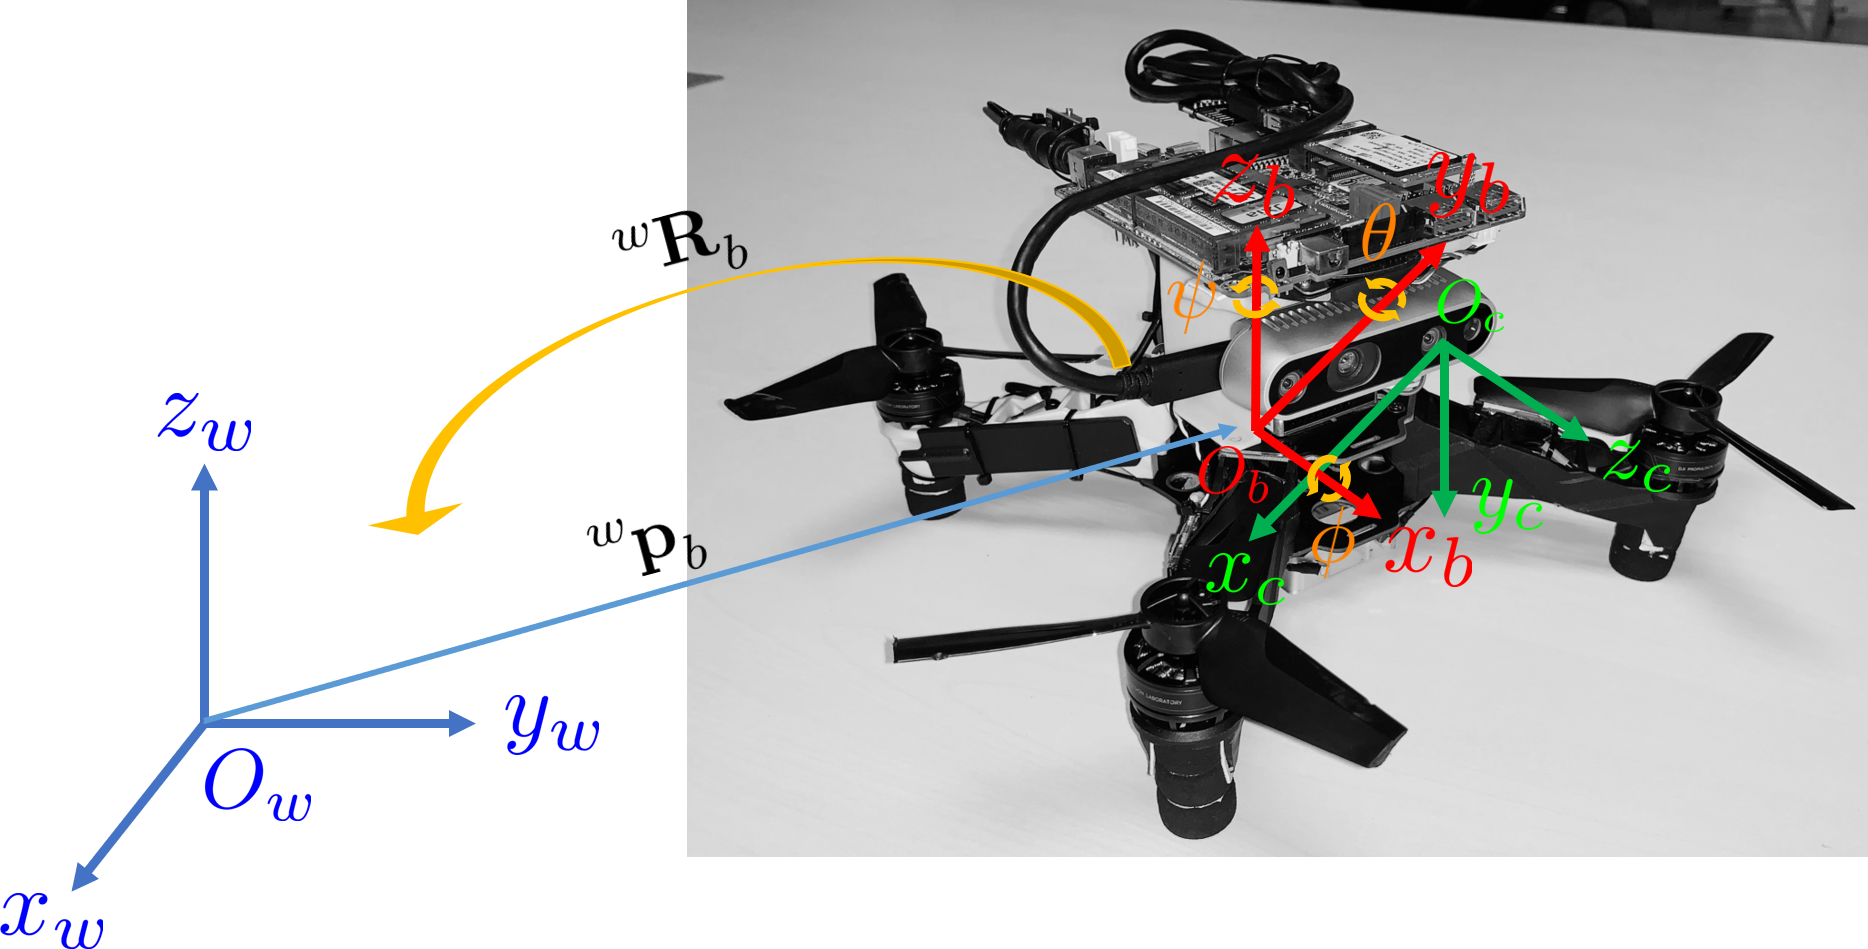
\includegraphics[width=1.0\textwidth]{figure/chapter_4/coordinate.png}
  \caption{Coordinate frames of world, UAV body and on-board camera}
  \label{fig:coordinate}
\end{figure}

Three coordinate frames are considered in our flocking system including the world, UAV body and on-board camera frames, as illustrated in Fig.\ref{fig:coordinate}. In Ch.\ref{tracking}, the target UAV is first captured in camera frame denoted by $\mathbf{p_c}\in\mathbb{R}^3$, then for the simplicity and unity of the calculations, $\mathbf{p_c}$ is transformed back to world frame $\mathbf{p_w}\in\mathbb{R}^3$ by $\tensor*[^w]{\mathfrak{g}}{_c}\in\mathbb{R}^{4\times4}$:

\begin{equation}\label{eq:transform}
\begin{aligned}
\begin{bmatrix}\mathbf{p^T_w}&1\end{bmatrix}^T&=\tensor*[^w]{\mathfrak{g}}{_c}\begin{bmatrix}\mathbf{p^T_c}&1\end{bmatrix}^T\\
\tensor*[^w]{\mathfrak{g}}{_c}&=\tensor*[^w]{\mathfrak{g}}{_b}\tensor*[^b]{\mathfrak{g}}{_c}=\begin{bmatrix}\mathbf{\tensor*[^w]{R}{_b}}&\mathbf{\tensor*[^w]{p}{_b}}\\\mathbf{0^{1\times3}}&1\end{bmatrix}
\begin{bmatrix}\mathbf{\tensor*[^b]{R}{_c}}&\mathbf{\tensor*[^b]{p}{_c}}\\\mathbf{0^{1\times3}}&1\end{bmatrix}\\
\tensor*[^b]{\mathbf{R}}{_c}&=\mathbf{R_z}(\psi)\mathbf{R_y}(\theta)\mathbf{R_x}(\phi)
\end{aligned}
\end{equation}

\noindent
where $\mathbf{p_c}$ is first rotated w.r.t $z_c$ by yaw angle $\psi$, then $z_y$ by pitch angle $\theta$, last $z_x$ by roll angle $\phi$ and shifted by $\tensor*[^b]{\mathbf{p}}{_c}$ to $\mathbf{p_b}$ in body frame. Iteratively, $\mathbf{p_c}$ is transformed back to $\mathbf{p_W}$ in world frame (\ref{eq:transform}). It is worthwhile to point out that both $\tensor*[^b]{\mathfrak{g}}{_c}$ and $\tensor*[^w]{\mathfrak{g}}{_b}$ are estimated online by the method developed in~\cite{VINS}. The $\mathbf{R_z}(\psi)$, $\mathbf{R_y}(\theta)$ and $\mathbf{R_x}(\phi)\in\mathfrak{SE(3)}$ are rotation matrixes:

\begin{equation}\label{eq:rotation}
\begin{aligned}
R_z(\psi)&=\begin{bmatrix}cos\psi&-sin\psi&0\\sin\psi&cos\psi&0\\0&0&1\end{bmatrix}\\
R_y(\theta)&=\begin{bmatrix}cos\theta&0&sin]\theta\\0&1&0\\-sin\theta&0&cos\theta\end{bmatrix}\\
R_x(\phi)&=\begin{bmatrix}1&0&0\\0&cos\phi&-sin]\phi\\0&sin\phi&cos\phi\end{bmatrix}
\end{aligned}
\end{equation}

\subsection{UAV Dynamics and Kinematics}

We denote the center of mass of UAV body in world frame by $\mathbf{r}\in\mathbb{R}^3$, then from Newton's law we have:

\begin{equation}\label{eq:newton}
m\mathbf{\ddot{r}}=\begin{bmatrix}0\\0\\-mg\end{bmatrix}+\tensor*[^w]{\mathbf{R}}{_b}\begin{bmatrix}0\\0\\\sum F_i\end{bmatrix}
\end{equation}

where $\mathit{m}\in\mathbb{R}$ is the total weight of the UAV and $\mathit{F_i}\in\mathbb{R}$ is the lifting force provided by each motor. The components of the angular velocities of UAV in its body frame are denoted by $\mathit{p}$, $\mathit{q}$ and $\mathit{r}\in\mathbb{R}$ and are related with $\theta$, $\phi$ and $\psi\in\mathbb{R}$ by:

\begin{equation}\label{eq:pqr}
\begin{bmatrix}p\\q\\r\end{bmatrix}=\begin{bmatrix}cos\theta&0&-cos\phi sin\theta\\0&1&sin\phi\\sin\theta&0&cos\phi cos\theta\end{bmatrix}\begin{bmatrix}\dot{\phi}\\\dot{\theta}\\\dot{\psi}\end{bmatrix}
\end{equation}

In addition to force, each motor has also produced moment, $\mathit{M_i}\in\mathbb{R}$, perpendicular to $x_b-x_y$ plane. We denote the length from each motor to the center of mass by $\mathit{L}\in\mathbb{R}$ and the moment of inertia matrix along $x_b-y_b-z_b$ axes by $\mathbf{I}\in\mathbb{R}^{3\times3}$. We then have the following Euler equations:

\begin{equation}\label{eq:euler}
\mathbf{I}\begin{bmatrix}\dot{p}\\\dot{q}\\\dot{r}\end{bmatrix}=\begin{bmatrix}L(F_2-F_4)\\L(F_3-F_1)\\M_1-M_2+M_3-M_4\end{bmatrix}-\begin{bmatrix}p\\q\\r\end{bmatrix}\times
\mathbf{I}\begin{bmatrix}p\\q\\r\end{bmatrix}
\end{equation}

As shown in Fig.\ref{fig:nest}, the control loops are divided into inner attitude control and outer position control. With the help of DJI Onboard SDK and owing to the differential flatness property, the state and input could be represented as algebraic functions of four carefully selected flat outputs $[\mathbf{r}^T, \psi]$ and their derivatives~\cite{Snap}. This facilitates the generation of trajectories since any smooth trajectory (with reasonably bounded derivatives) in the space of flat outputs can be followed by the UAV. In Ch.\ref{tracking}, the main work of chaser UAV's motion planning goes to the design of the required trajectory.

\begin{figure}[htb]
  \centering
  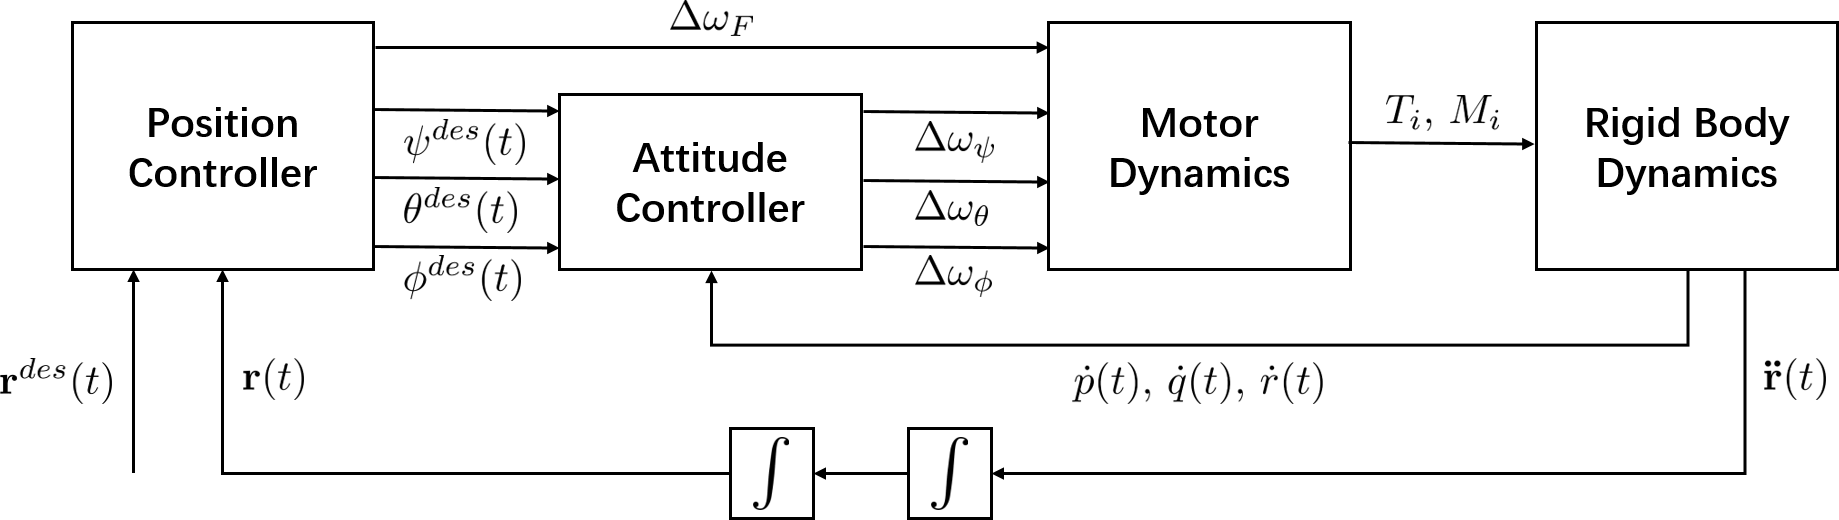
\includegraphics[width=1.0\textwidth]{figure/chapter_2/nest.png}
  \caption{Nested control loops for position and attitude control,~\cite{GRASP}}
  \label{fig:nest}
\end{figure}

\section{Hardware architecture}\label{hardware}

The hardware platform of our flocking system includes one follower UAV, one leader UAV and their remote controllers (RCs) as shown in Fig.\ref{fig:quadrotor_controller} and Fig.\ref{fig:target_uav}. The leader UAV is fully manually controlled and the follower UAV is first controlled by the RC to take off, then the control authority is switched to the on-board mini computer and achieve autonomous driving. The RC is designed to have higher control authority than the on-board computer that human operator could prevent the UAV from fatal errors by switching control priority back to RC.

\begin{figure}[ht]
  \centering
  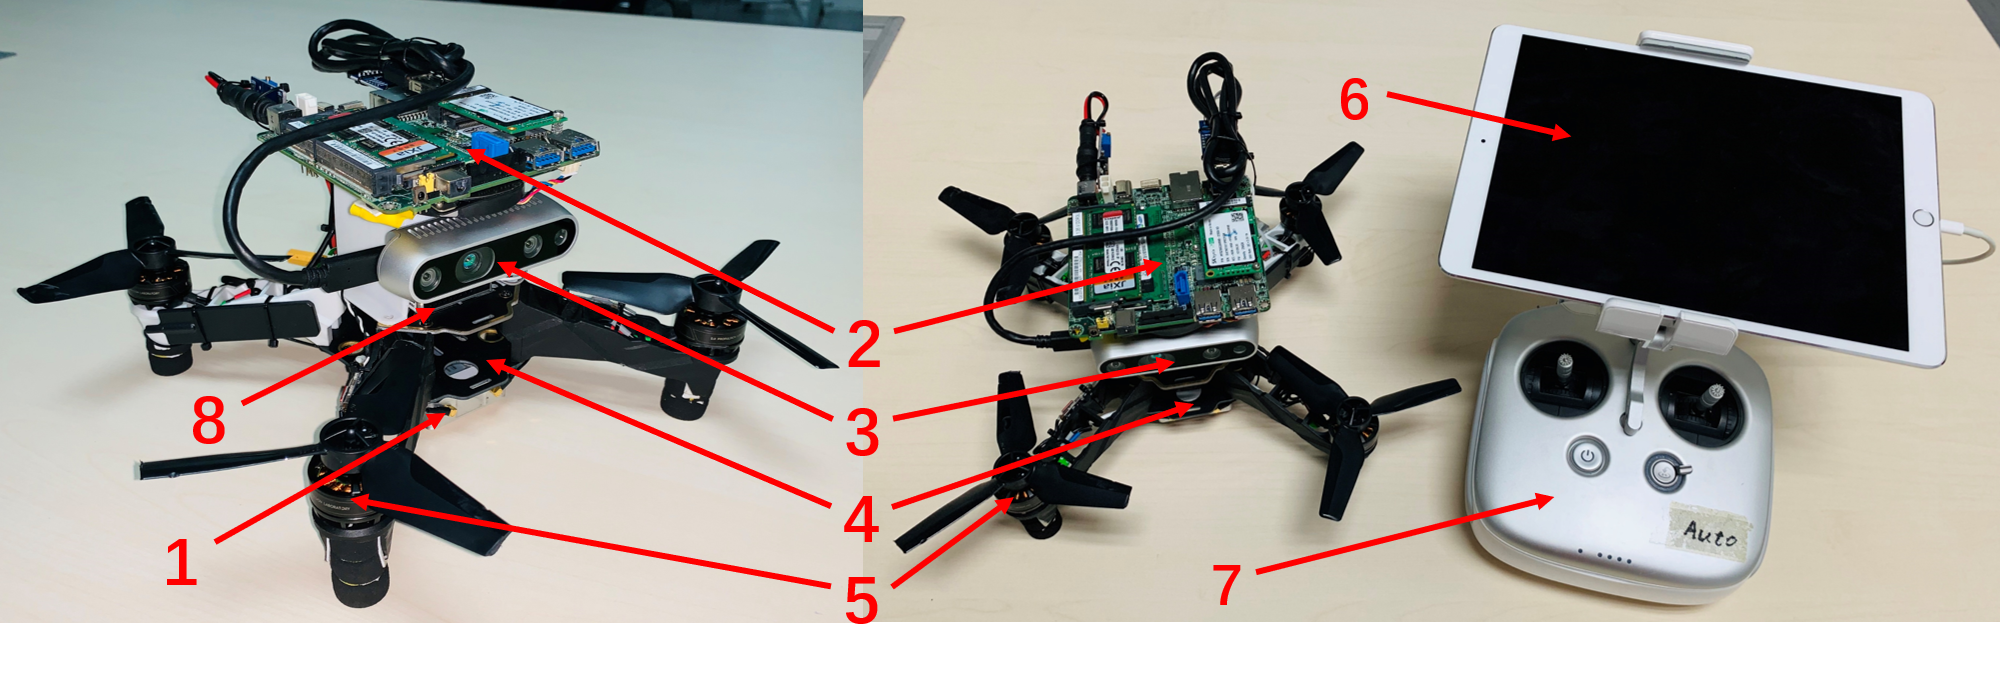
\includegraphics[width=1.0\textwidth]{figure/chapter_4/chaser_intro.png}
  \caption{Follower UAV and remote controller panel: (1) Lightbridge 2 receiver; (2) Intel NUC mini computer; (3) Intel Realsense camera; (4) 4S LiPo Batter Case; (5) DJI snail motor; (6) iPad Live streaming panel; (7) DJI Lightbridge 2 remote controller; (8) DJI N3 flight controller.}
  \label{fig:quadrotor_controller}
\end{figure}

\begin{figure}[htb]
  \centering
  \subfigure[Look from the back, with unique aruco code.]{\label{fig:back}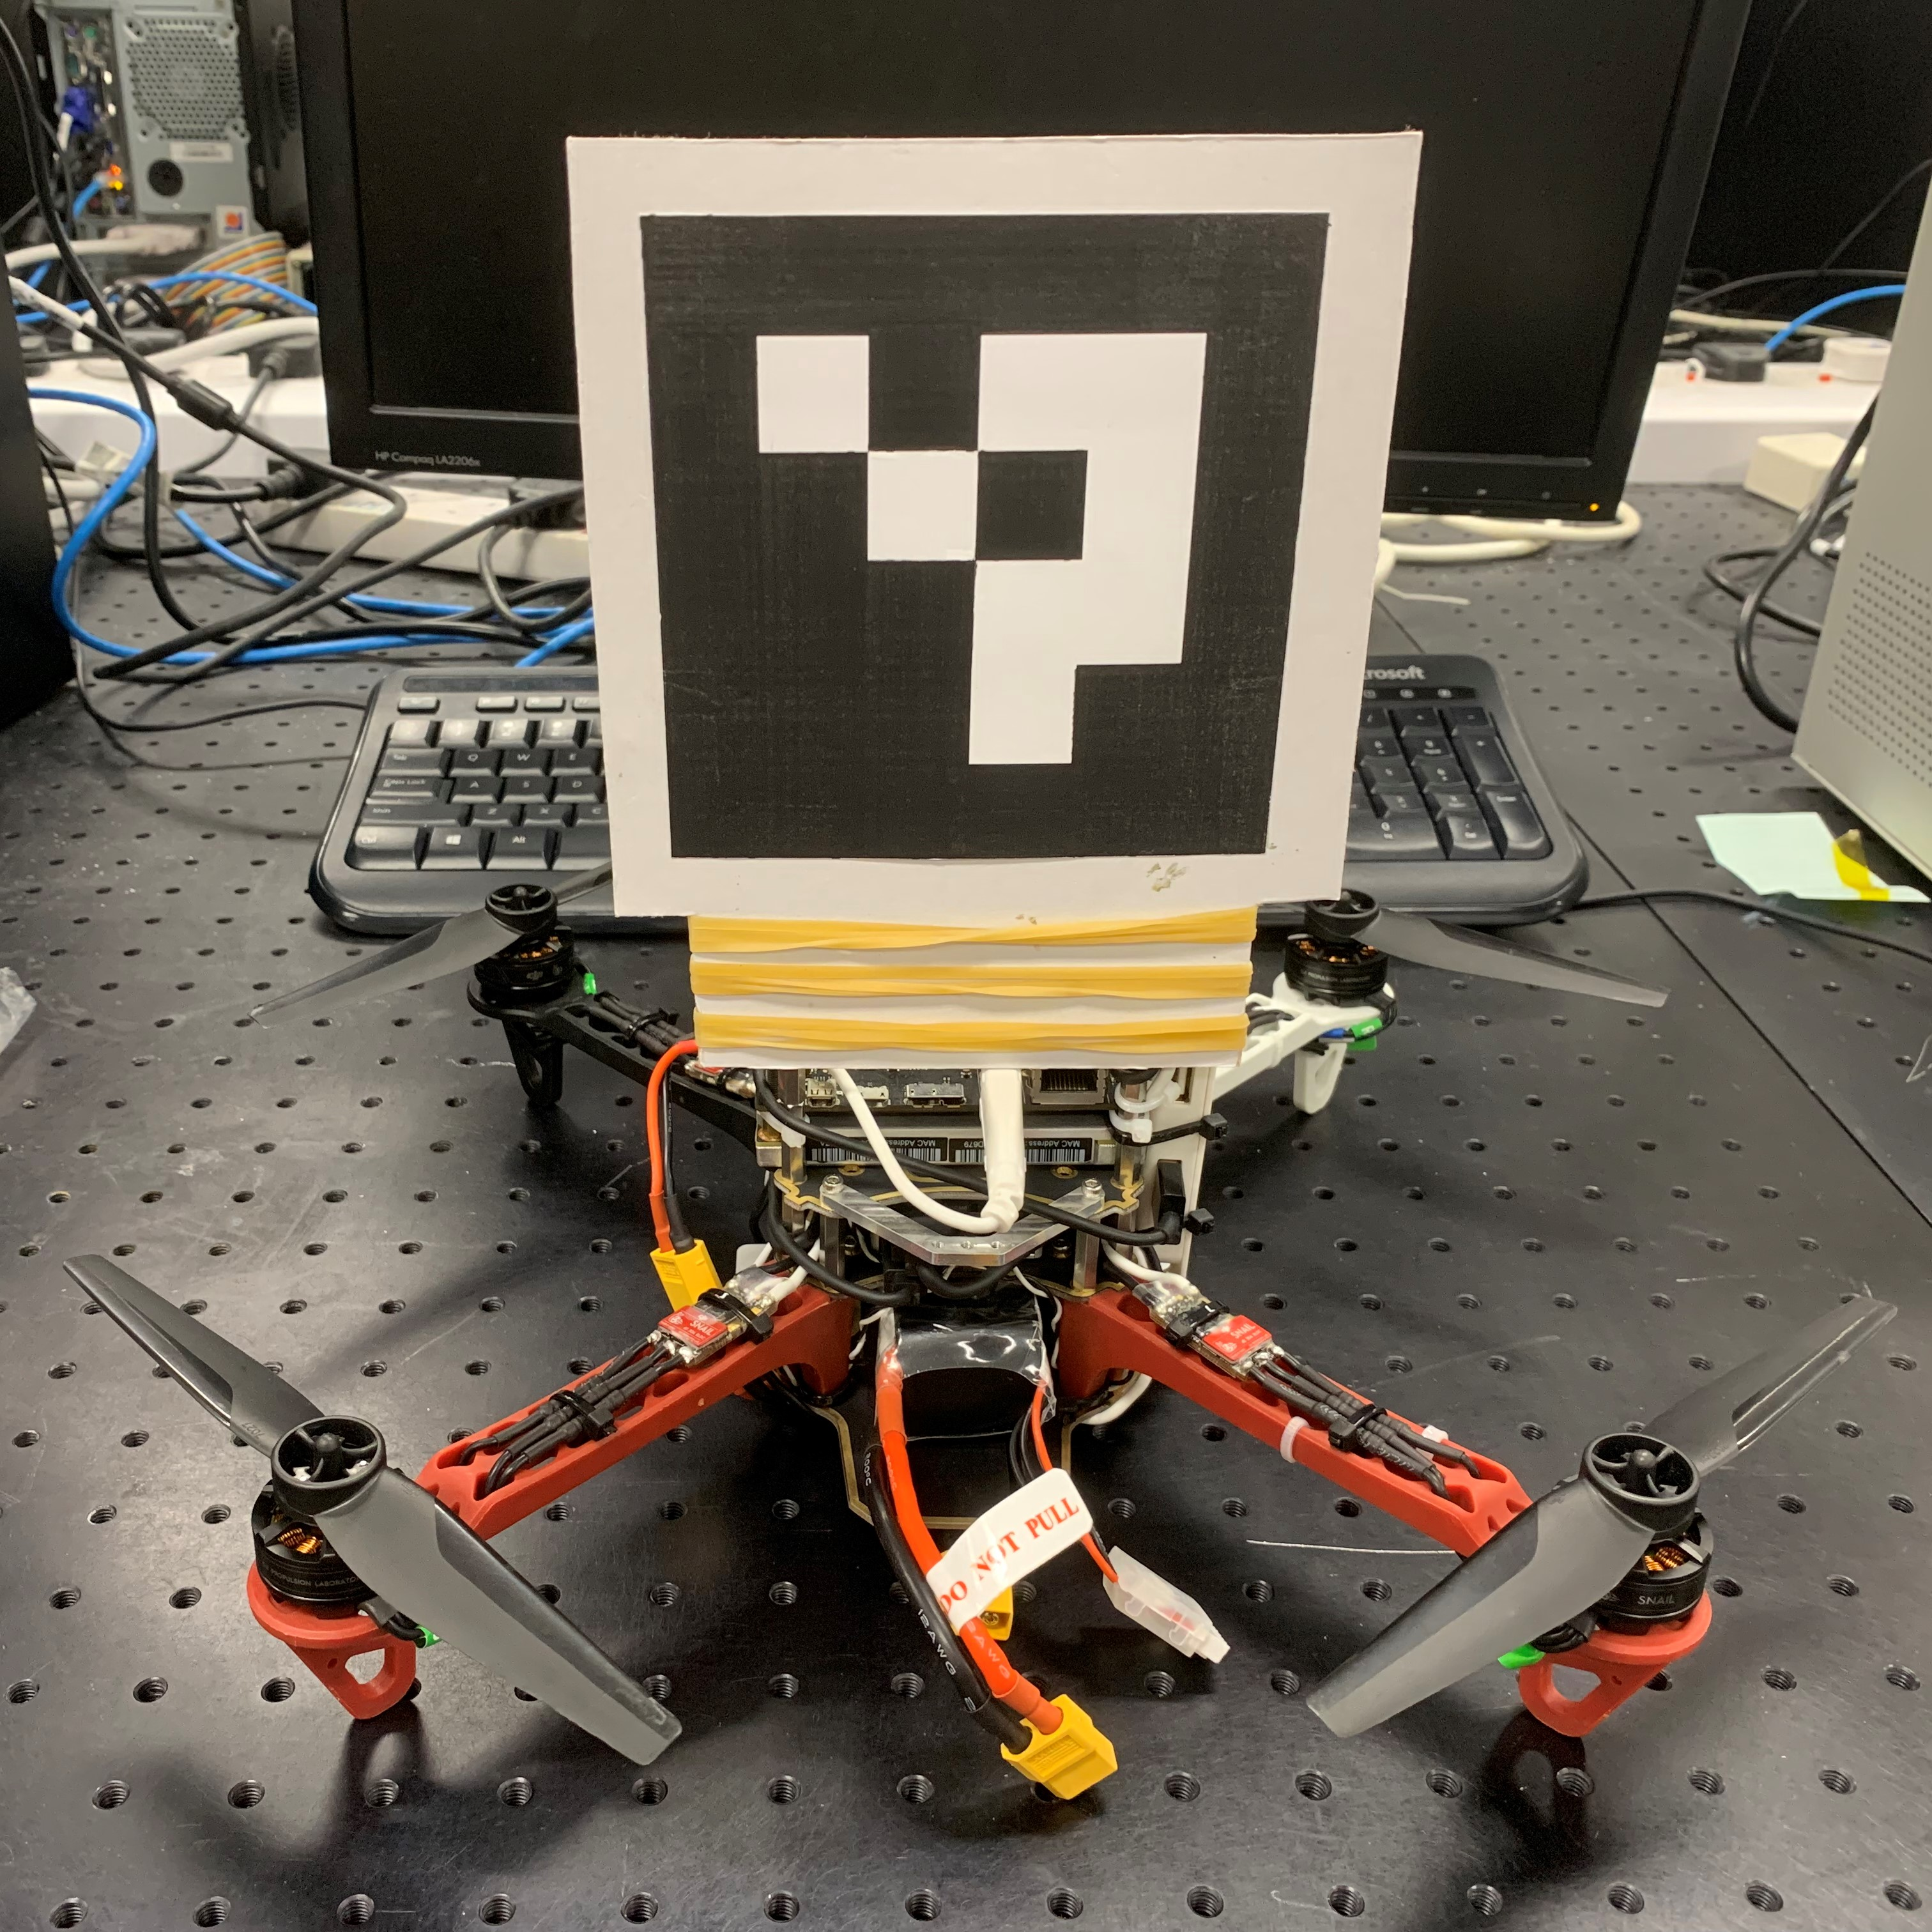
\includegraphics[width=0.49\textwidth]{figure/chapter_4/leader_back.jpg}}
  \subfigure[Look from the front, with Guidance system mounted.]{\label{fig:front}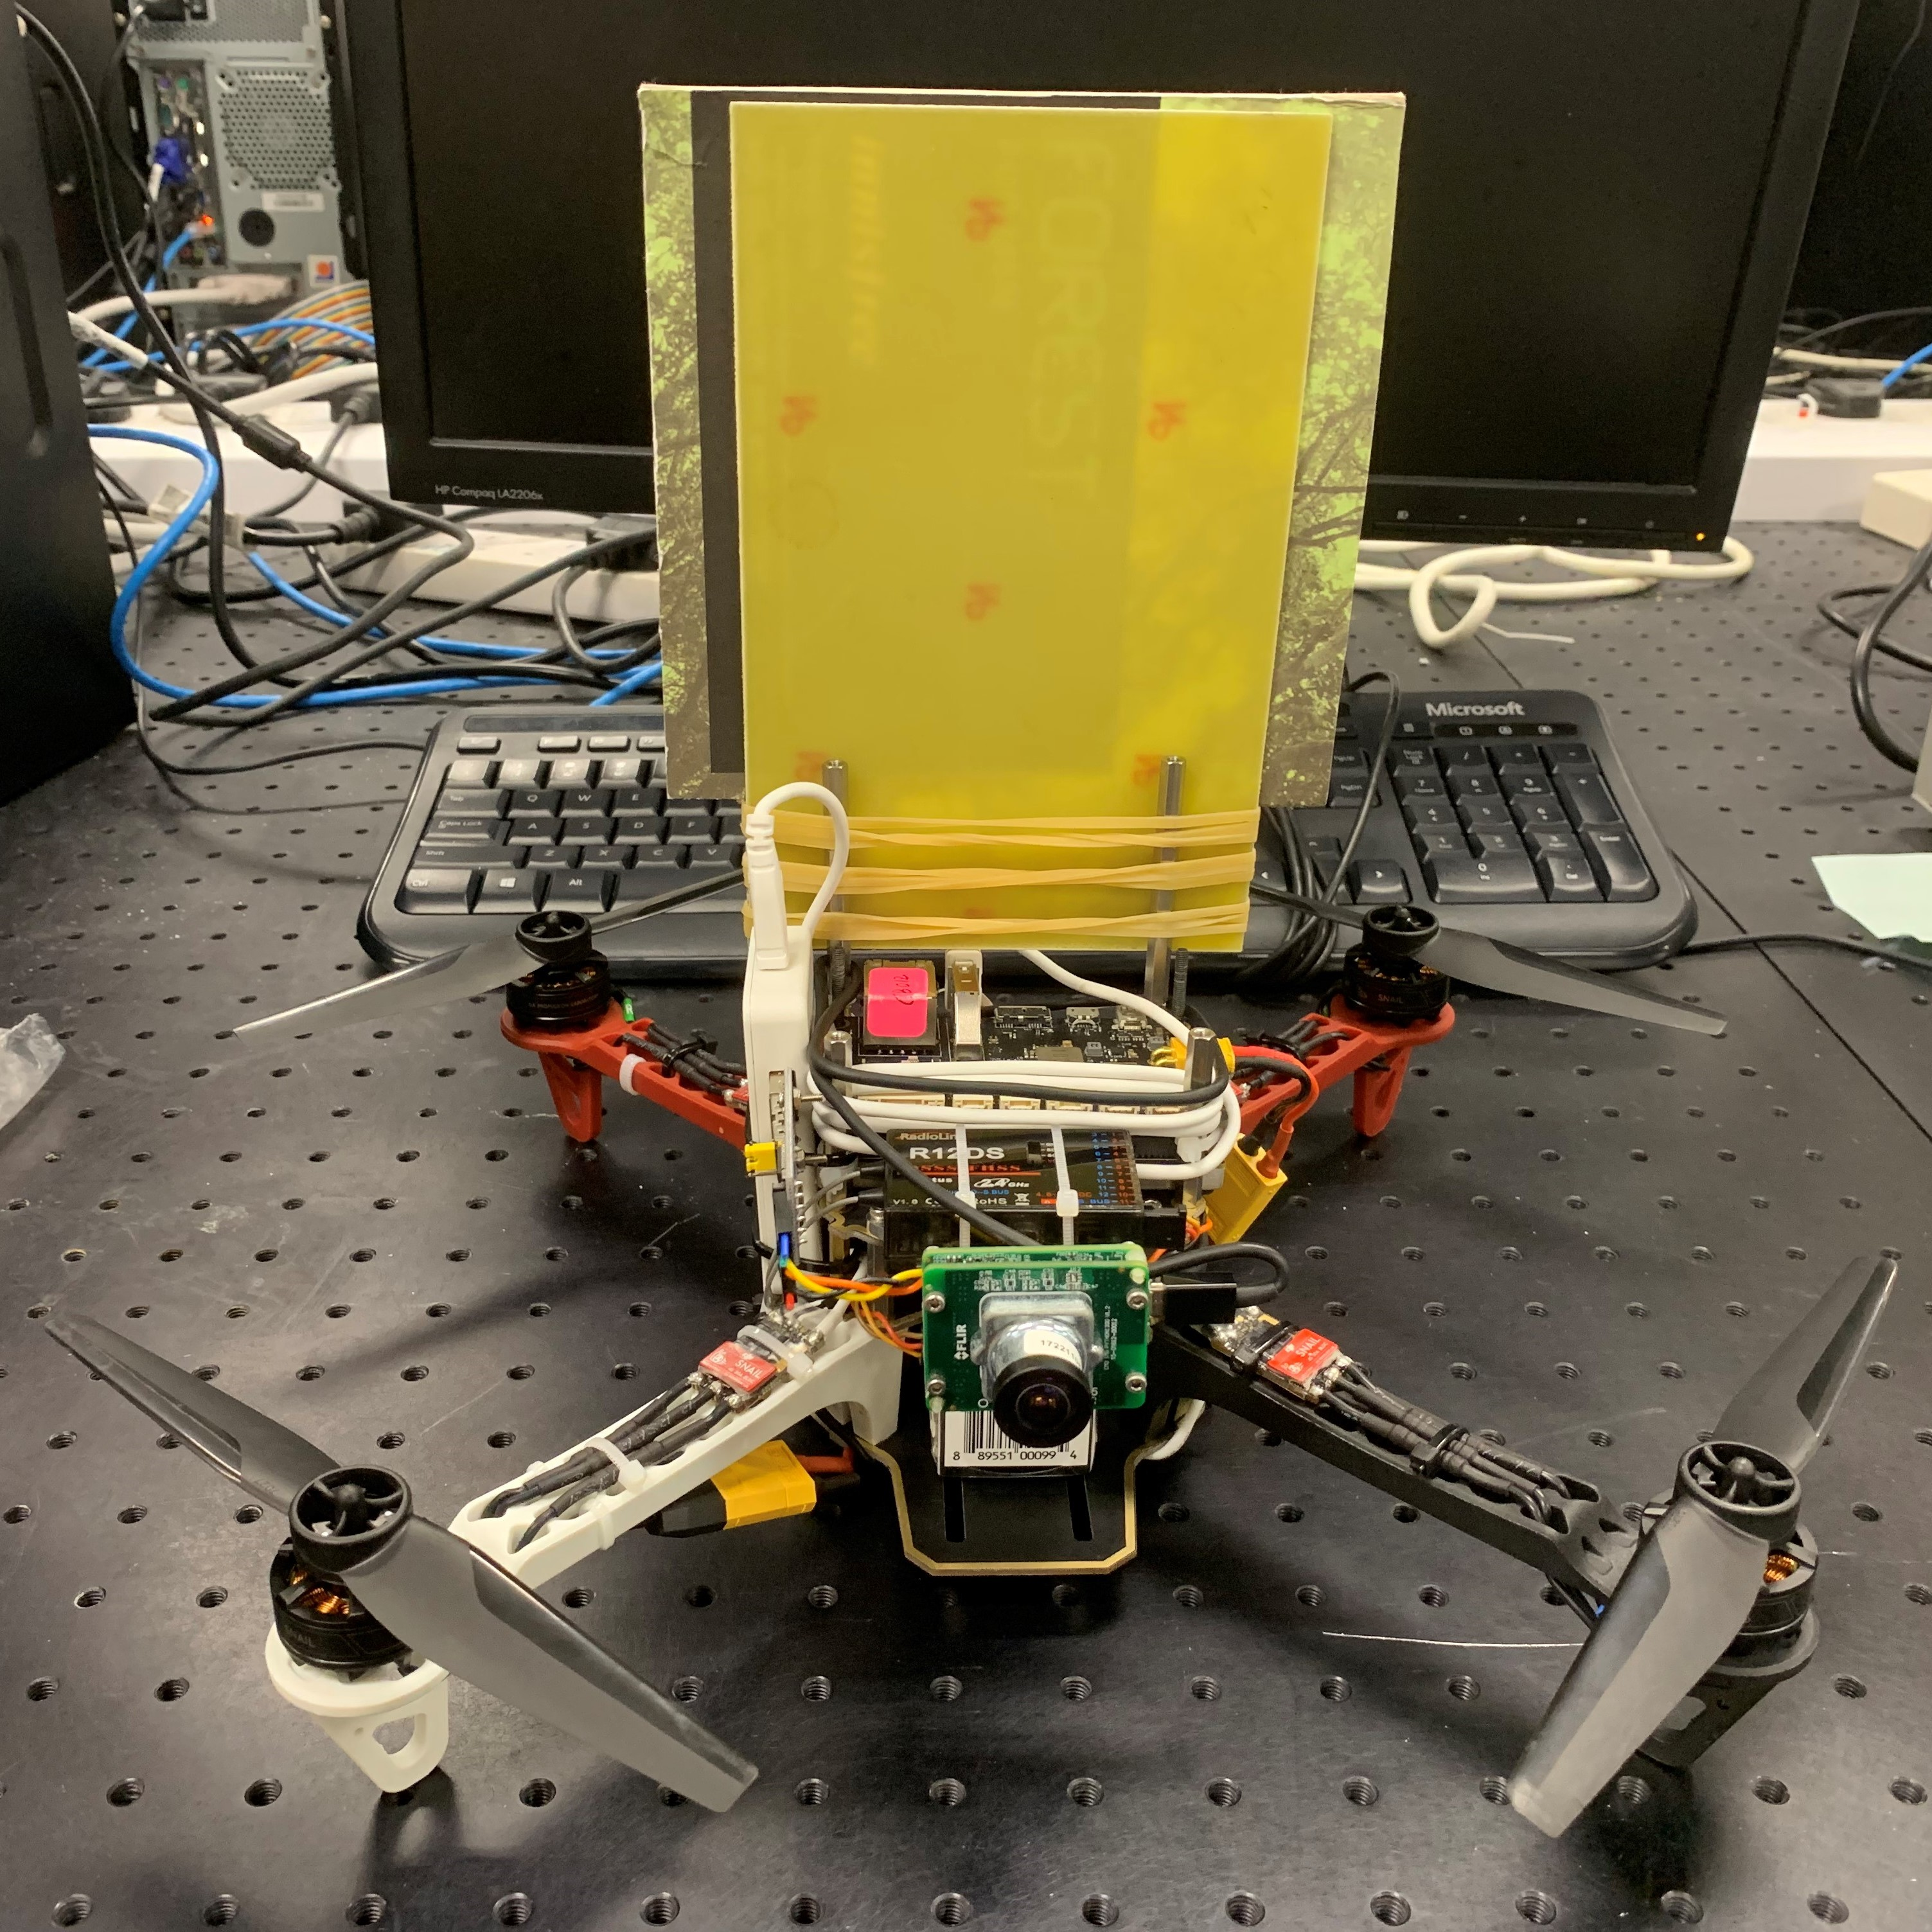
\includegraphics[width=0.49\textwidth]{figure/chapter_4/leader_front.jpg}}
  \caption{Leader UAV.}\label{fig:target_uav}
\end{figure}

\begin{table}[htb]
  \centering
 \linespread{1.7}{ {\footnotesize
\vspace{2em}
  \begin{tabular}{ccc}
  \hline
\noalign{\smallskip}
  \textbf{Component} & \textbf{Weight(g)} & \textbf{Power(W)}\\
\noalign{\smallskip}
  \hline
  Intel NUC i5 mini computer & 125 & 15(avg) \\
  Intel Realsense D435i camera & 272 & 2.5(avg) \\
  DJI N3 flight controller & 92 & 3.3(avg)/5(peak) \\
  DJI Lightbridge 2 receiver & 70 &  7.8(avg)\\
\noalign{\smallskip}
  \hline
  \end{tabular}
  }}
  \caption{Weight and power consumption of components on the follower UAV.}
  \label{tb:weight_power}
\end{table}

\begin{figure}[ht]
  \centering
  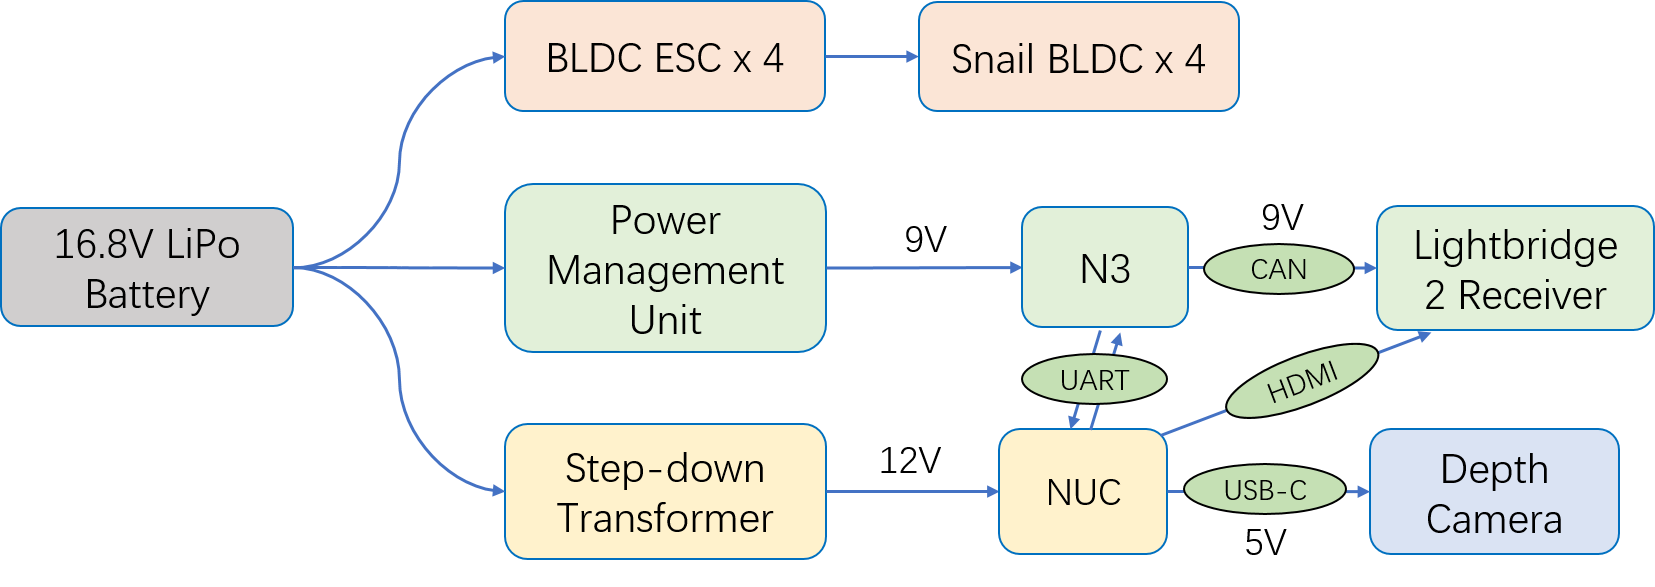
\includegraphics[width=1.0\textwidth]{figure/chapter_4/power_system.png}
  \caption{On-board power systems.}
  \label{fig:power_systems}
\end{figure}

The UAV frame consists of the mechanical construction, motors, propellers and the power supply module. Q250 is chosen as the follower UAV's frame for its compact size, firm material and the flexibility in maneuvering in cluttered environment. DJI snail BLDC motors and 5-inch 3-blade propellers are mounted for their racing optimized propulsion system and rapid response time. 4S LiPo battery is selected for on-board power supply for its 16.8 V output, 4200 mAh capacity and rechargeable property. The detailed follower UAV's on-board power supply system is illustrated in Fig.\ref{fig:power_systems}. The total weight including the battery is 1.12 kg and the diagonal length is 25 cm. We use Intel NUC i5 mini computer as our follower UAV's on-board computing resource for both frontend processing and backend optimization (Ch.\ref{tracking}). We choose Intel Realsense Depth camera D435i as the forward looking camera for both perception and leader UAV feature recognition. It is outfitted with a stereo global shutter camera, with resolution up to 1920x1080 pixels, frame rate up to 90 FPS and direct depth map output. With sufficient tests, only the left monocular camera is employed to balance the power consumption. More details about on-board components can be found in Table~\ref{tb:weight_power}.

The overall system stability is more emphasized than flexibility on leader UAV, where F330 frame with diagonal length of 33 cm, DJI 2312E BLDC motors, 7-inch propellers and the DJI Guidance vision-feedback position system are mounted. With Guidance system and its built-in ultrasonic sensor, it is easier for the leader UAV to hover and maneuver at a fixed height. The demand for computation and perception capability on leader UAV is lower than the follower, as its flight path is controlled by human operator, thus it is not embedded with any external processor. DJI N3 flight controllers are selected for both follower and leader UAVs, due to their high quality built-in IMU sensor and compatibility with DJI Lightbridge 2 for live streaming.

\section{Software architecture}\label{software}

\begin{figure}[ht]
  \centering
  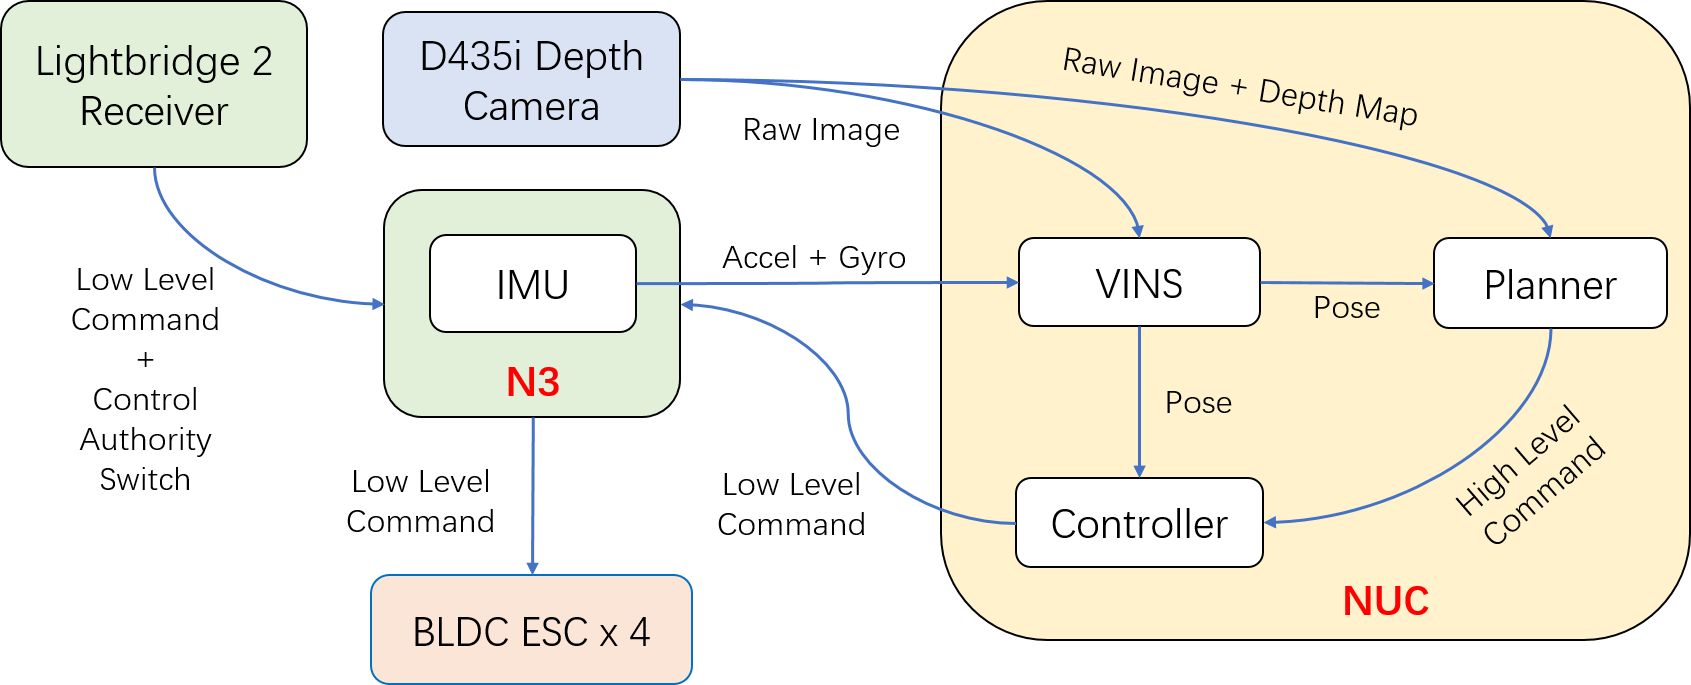
\includegraphics[width=1.0\textwidth]{figure/chapter_4/system_diagram.png}
  \caption{Software architecture}
  \label{fig:software_architecture}
\end{figure}

The software architecture is shown in Fig.\ref{fig:software_architecture}. On the follower's mini i5 computer, 400 Hz IMU measurements and 30 Hz grey scale image data are fused in the visual-inertial state estimator~\cite{VINS} to obtain UAV self position and orientation. Unique aruco code~\cite{Aruco} is attached on leader UAV to simplify the relative displacement and pose estimation. Unlike many existing flocking systems that rely on motion capture system (VICON), global positioning system (RTK) or LiDAR, our follower UAV only utilizes forward looking monocular camera for state estimation to maximally imitate natural birds. We show through both indoor and outdoor experiments that our minimal sensing setup is sufficient for the realization of our flocking model with Algorithm~\ref{alg:a1}.

\begin{algorithm}[h]
  \caption{Flocking algorithm for the follower UAV}
  \label{alg:a1}
  \begin{algorithmic}[1]
    \If{flocking signal triggered}
      \State estimate body pose, capture leader's image;
      \While {new image}
        \State estimate relative displacement $\mathit{x_i-x_j}$;
        \State calculate relative velocity $\mathit{v_i-v_j}$ from differentiation;
        \State calculate desired acceleration $\mathit{u_i}$ from proposed model;
        \State execute flocking command;
      \EndWhile
    \EndIf
  \end{algorithmic}
\end{algorithm}

We have also utilized DJI Lightbridge 2 for remote debugging and monitoring. The Lightbridge 2 transforms mini computer's desktop stream to iPad Pro for visualization, including current leader UAV's pose and live image processing output. This enables us to remotely manipulate the on-board computer while the UAV is in the air.

\newpage
